%; whizzy chapter
% -initex iniptex -latex platex -format platex -bibtex jbibtex -fmt fmt
% 以上 whizzytex を使用する場合の設定。

%     Kansai Debian Meeting resources
%     Copyright (C) 2007 Takaya Yamashita
%     Thank you for Tokyo Debian Meeting resources

%     This program is free software; you can redistribute it and/or modify
%     it under the terms of the GNU General Public License as published by
%     the Free Software Foundation; either version 2 of the License, or
%     (at your option) any later version.

%     This program is distributed in the hope that it will be useful,
%     but WITHOUT ANY WARRANTY; without even the implied warranty of
%     MERCHANTABILITY or FITNESS FOR A PARTICULAR PURPOSE.  See the
%     GNU General Public License for more details.

%     You should have received a copy of the GNU General Public License
%     along with this program; if not, write to the Free Software
%     Foundation, Inc., 51 Franklin St, Fifth Floor, Boston, MA  02110-1301 USA

%  preview (shell-command (concat "evince " (replace-regexp-in-string "tex$" "pdf"(buffer-file-name)) "&"))
% 画像ファイルを処理するためにはebbを利用してboundingboxを作成。
%(shell-command "cd image200708; ebb *.png")

%%ここからヘッダ開始。

\documentclass[mingoth,a4paper]{jsarticle}
\usepackage{kansaimonthlyreport}
\usepackage[dvipdfmx]{xy}
\usepackage{etex}
\usepackage{ulem}

% 日付を定義する、毎月変わります。
\newcommand{\debmtgyear}{2014}
\newcommand{\debmtgdate}{28}
\newcommand{\debmtgmonth}{9}
\newcommand{\debmtgnumber}{88}

\def\fixme#1{{\color{red}{#1}}}

\begin{document}

\begin{titlepage}

% 毎月変更する部分、本文の末尾も修正することをわすれずに

 第\debmtgnumber{}回 関西 Debian 勉強会資料

\vspace{2cm}

\begin{center}
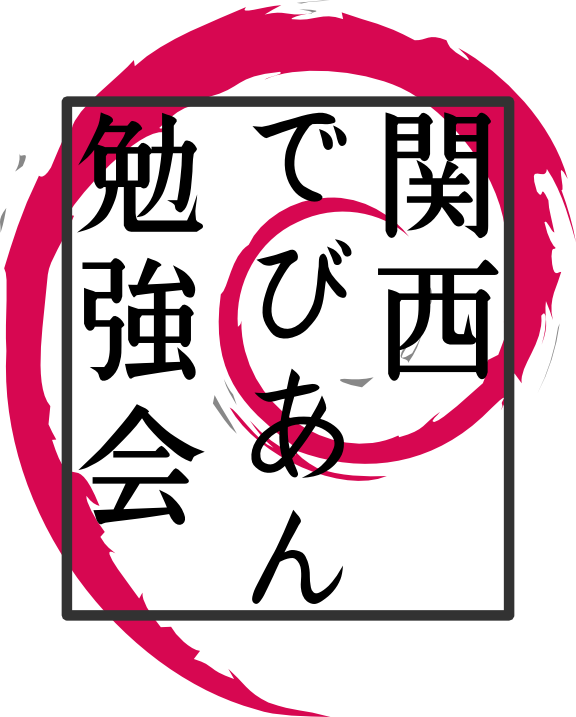
\includegraphics{image200802/kansaidebianlogo.png}
\end{center}

\begin{flushright}
\hfill{}関西 Debian 勉強会担当者 佐々木・倉敷・のがた・かわだ・八津尾 \\
\hfill{}\debmtgyear{}年\debmtgmonth{}月\debmtgdate{}日
\end{flushright}

\thispagestyle{empty}
\end{titlepage}

\dancersection{Introduction}{Debian JP}

\vspace{1em}

 関西Debian勉強会はDebian GNU/Linuxのさまざまなトピック
 (新しいパッケージ、Debian特有の機能の仕組、Debian界隈で起こった出来事、
 などなど)について話し合う会です。

 目的として次の三つを考えています。
 \begin{itemize}
  \item MLや掲示板ではなく、直接顔を合わせる事での情報交換の促進
  \item 定期的に集まれる場所
  \item 資料の作成
 \end{itemize}

 それでは、楽しい一時をお過ごしください。

\newpage

\begin{minipage}[b]{0.2\hsize}
 {\rotatebox{90}{\fontsize{80}{80}
{\gt 関西 Debian 勉強会}}}
\end{minipage}
\begin{minipage}[b]{0.8\hsize}
\hrule
\vspace{2mm}
\hrule
\setcounter{tocdepth}{1}
\tableofcontents
\vspace{2mm}
\hrule
\end{minipage}

\dancersection{最近のDebian関係のイベント報告}{Debian JP}

\subsection{第87回関西Debian勉強会}

87回目の関西Debian勉強会は8月24日(日)に、港区民センターで行なわれました。

もくもくの会を中心とした内容での開催でした。

kozo2さんから投げかけられた、iron-maiden-clのパッケージ化、cmakeでのdeb
パッケージ作成、travisでの勉強会資料の作成といった話題をみなさんであれ
これとしていました。

travisでの勉強会資料の作成は、資料をビルドできるdockerのコンテナに入れ
るようにして、Docker Hubでbuild detailをみるというところに落ち着いたよ
うです。
\footnote{\url{https://registry.hub.docker.com/u/kozo2/debian-monthly-report/}}

\begin{commandline}
$ docker run -i -t kozo2/debian-monthly-report /bin/bash
\end{commandline}

\subsection{第117回東京エリアDebian勉強会}

117回目の東京エリアDebian勉強会は9月26日(土)に株式会社スクウェア・エニッ
クス セミナールームで開催されました。

野島さんによる「Debconf14のビデオ紹介」ともくもくの会で開催されました。

\subsection{Debian Project}

\subsubsection{DebConf14}

Debian Conference 2014\footnote{\url{http://debconf14.debconf.org/}}
がアメリカのオレゴン州ポートランドで8/23(土)〜8/31(日)の間開催されまし
た。

当初の予定にはなかった、Linus Toravaldsさんがゲストとして呼ばれ
「Q\&A with Linus Torvalds」
\footnote{\url{https://summit.debconf.org/debconf14/meeting/155/qa-with-linus-torvalds/}}
のセッションが開催されました。

日本からは、g新部(gniibe)さんとやまね(henrich)さんが参加されていました。

先日の東京エリアDebian勉強会でセッションのビデオ試聴方法や書き起こしテ
キストが紹介されていますので参照してください。

次回のDebConf15はドイツのハイデルベルグにて2015年8月15日から22日にかけ
て開催される予定です。


\subsubsection{John Paul Adrian Glaubitzさん来日}

ドイツのDebian DeveloperであるJohn Paul Adrian Glaubitz(glaubitz)さんが
来日されましたので、関西では野方が姫路城を案内し、後日、倉敷、野方、か
わだで迎撃しました。

GlaubitzさんはNintendo64など日本のコンシューマゲームが好きなナイスガイ
でした。楽しい一時を過ごしつつキーサインを行ないました。


\subsubsection{``shellshock'' bugs}

秋のbash祭りとして世間を騒がせているshellshockバグことCVE-2014-6271です
が、セキュリティアドバイザリが出ていますので忘れずにUpdateしましょう。

はじめに出されたDSA-3032-1だけでは対策が不十分でしたので、その後
DSA-3035-1が出されました。こちらが適用されているか確認してください。
CVE-2014-6271の問題だけでなくCVE-2014-7169の問題も修正されています。


\dancersection{事前課題}{Debian JP}

今回の課題は以下の通りです。
\begin{screen}
  \begin{enumerate}

  \item %
    もくもくの会で行なう作業、質問などの課題を用意して教えてください。
    (電源とネットワーク(WiMAXなど)はありますが、それ以外の作業に必要な
    環境はご用意ください。)

  \item %
    前回(第87回)の勉強会に参加された方は、前回の作業や課題がその後どう
    なったか結果を教えてください。

  \item %
    LT(ライトニングトーク) 歓迎です。何かお話したい方はタイトルを下さい。

  \end{enumerate}
\end{screen}

参加者の皆さんの解答は以下の通りです:

\begin{prework}{ 木下 }
  \begin{enumerate}
  \item
    \begin{enumerate}
    \item プライベートクラウドの調査・研究
      \begin{itemize}
      \item Openstackの研究
      \item Eucalyptusの研究/実験
      \end{itemize}
    \item グリッドコンピューティング関連の調査・研究
      \begin{itemize}
      \item GlobusToolkitで何ができる?

        →AndroidOS等のJavaVMのコンパイルで使えたら嬉しいかも。
      \end{itemize}
    \item Debian7 on PANDABOARDの調査・研究
      \begin{itemize}
      \item WiFiモジュール(On Board:TI製)の有効化
      \item GPUデバイスドライバの有効化
      \end{itemize}
    \end{enumerate}
  \item ※欠席だった為割愛
  \end{enumerate}
\end{prework}

\begin{prework}{ かわだてつたろう }
後で。。。
\end{prework}

\begin{prework}{ 佐々木洋平 }
tDiary...
\end{prework}

\begin{prework}{ murase\_{}syuka }
  \begin{itemize}
  \item mrubyのパッケージ更新
  \item blenderのビルド
    \begin{itemize}
    \item openimageioでboostがエラー
    \end{itemize}
  \item emacs弄る
  \item etc
  \end{itemize}
\end{prework}

\begin{prework}{ Mitsutoshi NAKANO $<$bkbin005@rinku.zaq.ne.jp$>$ }
  \begin{enumerate}
  \item 以下のうち、いずれか。
    \begin{enumerate}
    \item Debian のパッケージビルドの方法についての勉強
    \item canna-yubinを拡張し、FreeWnnに対応させる。

      \url{http://sourceforge.jp/projects/freewnn/lists/archive/users/2014-August/000211.html}

      \url{http://sourceforge.jp/projects/canna-yubin/}
    \item しばらくNetにアクセスできない可能性が出てきたので、関係各所への連絡の文案を考える。
    \end{enumerate}
  \item
    \begin{enumerate}
    \item tamago の upstream の準備

      tamagoの大元の開発者である戸村さんと連絡が取れました。

      戸村さんより

      \begin{quote}
      tamago については、勤務先の業務の一部として開発したことに
      なるはずなので、それ関連の手続きがどうなっているかなども
      確認しようとしているところでした。
      \end{quote}

      とのことで、権利関係の確認をしていただいております。

    \item Debian のパッケージビルドの方法についての勉強

      滞っています。
    \end{enumerate}
  \end{enumerate}
\end{prework}

\begin{prework}{ 山城の国の住人 久保博 }
とあるパッケージの不具合修正パッチが投げっぱなしになっている件について、ご相談させてください。
\end{prework}

\begin{prework}{ 川江 }
  \begin{enumerate}
  \item emacsを使った、JavascriptとCSSのコーティング。
  \item 苦戦中。ただし、やっとコードの全体像が読めてきた感じ(なぜに、fireFox、IE、Safari、Chromeは書式が違うのだろうか?もう少し「統一」してくれ!)
  \item なし
  \end{enumerate}
\end{prework}

\dancersection{もくもくの会}{}

\dancersection{今後の予定}{Debian JP}

\subsection{関西Debian勉強会}

次回、第89回関西Debian勉強会は10月26日(日)に港区民センターで開催予定で
す。

\subsection{東京エリアDebian勉強会}

第118回東京エリアDebian勉強会は10月18日(土)に開催予定です。
場所、内容については東京エリアDebian勉強会のウェブサイトを確認してくだ
さい。

%
% 冊子にするために、4の倍数にする必要がある。
% そのための調整
%% \dancersection{メモ}{}
%% \mbox{}\newpage
%% \mbox{}\newpage
%% \mbox{}\newpage

\printindex
%\cleartooddpage

 \begin{minipage}[b]{0.2\hsize}
  \rotatebox{90}{\fontsize{80}{80} {\gt 関西 Debian 勉強会} }
 \end{minipage}
 \begin{minipage}[b]{0.8\hsize}

 \vspace*{15cm}
 \rule{\hsize}{1mm}
 \vspace{2mm}
 
\includegraphics[width=2cm]{image200502/openlogo-nd.eps}
 \noindent \Large \bfseries{Debian 勉強会資料}\\ \\
 \noindent \normalfont \debmtgyear{}年\debmtgmonth{}月\debmtgdate{}日 \hspace{5mm}  初版第1刷発行\\
 \noindent \normalfont 関西 Debian 勉強会 (編集・印刷・発行)\\
 \rule{\hsize}{1mm}
 \end{minipage}

\end{document}
